\chapter{Design}

The purpose of the transactive module is to provide a proof of concept simulation of transactive control systems that span entire electricity interconnection. The simulation operates with a minimum timestep of 1 second and implements both balancing and frequency regulation services using real-time prices as the primary control signal and bids as the primary measurement signal throughout the system.

\section{Background}

The mismatch in the characteristic size, time, uncertainty of loads relative to generators of loads is a significant obstacle to using demand response to simultaneously displace generation-centric reliability services and mitigate generator market power: there are relatively few easily observed generators and their characteristic response times are relatively slow compared to overall system dynamics. Loads in contrast are far smaller, far more numerous, and for more difficult to observe but potentially far faster acting than the overall system dynamics.  

The Olympic \cite{hammerstrom2007} and Columbus \cite{widergren2014} demonstrations were successful in achieving their primary objectives, i.e., they used transactive control to show 1) that thermostatic demand resources could contribute to short-term capacity control using economic signals, and 2) that financial benefits would accrue to both utilities who installed and consumers who participated in such a control system.

Households recruited to participate in the Olympic and Columbus transactive control systems under the RTP tariff were equipped with home automation devices including a smart thermostat and a home-energy management system to integrate thermostats and other energy demand controllers with the utility metering system. The utility was equipped with a market-based dispatch system and communications links were established between the various components of the system.  For both the Olympic and Columbus experiments an operations plan was developed to test the system and observe the response to price fluctuations resulting from wholesale price variations, distribution congestion and critical peak pricing (CPP) events.

Various scenarios were designed to elicit demand response such that one could estimate the technical and economic properties of the transactive system. Various utility value streams such as peak-load capacity deferment, reduced wholesale power purchase costs and revenues from operating reserves markets were estimated. Consumer impacts such as benefit, surplus, comfort and billing impacts could then be recovered. The operating scenarios generally involved continually exposing customers to small fluctuations in price as well as changing feeder congestion limits at various times to induce large price changes.  The Olympic experiments were conducted from May 2006 to March 2007 in Clallam County and Port Angeles, Washington.  The Columbus experiments were conducted from June through September 2013 in the northeastern area of Columbus, Ohio. Various combinations of feeder congestion limits and durations were tested. These were selected at various time of day, day of week, and weather.  Additional critical-peak-pricing (CPP) responses were tested using selected CPP events. 

Households who were recruited to participate voluntarily to the Olympic Peninsula experiment were offered the choice of two new tariffs: a time-of-use (TOU) price or real-time price (RTP).  All customers received the same in-home equipment, including a smart thermostat and home-energy management wireless hub to establish connectivity to the utility's demand response dispatch system and provide 15-minute interval energy use metering. Some homes also received controllers for electric waterheaters and electric clothes dryers. Customers were then randomly assigned to the control group, a fixed price tariff, TOU or RTP. Regardless of the assignment, customers were promised on average \$150 benefit for participating 1 year. But they were told that the exact amount was uncertain and would be based on the tariff and how ``well'' they played the demand response ``game''. Customers were given an income based on their energy consumption prior to the announcement of the program to which an additional \$37.50 incentive was added quarterly. The monthly energy bills under the experiment tariff were then deducted from that income.  Any positive balance remaining at the end of each quarter was paid to them. During the experiment, customers continued to pay their normal bill to the utility and if customers overspent their quarterly income, they were not required to pay it back or carry the deficit into the following quarter. 

Columbus customers were recruited from a pool of homes that already had smart meters installed.  The smart meters provided 5 minute interval energy use data both to the utility's metering system and to the home energy management system, which was installed to maintain connectivity with the utility's demand response dispatch system. Customers were placed on an experimental RTP tariff approved by the Public Utility Commission of Ohio. Power was billed to consumers based on a commissioned-approved seasonal linear function of the wholesale LMP, plus feeder congestion costs, less a congestion rebate or a demand responsive incentive payment.  All other taxes and fees remained unchanged. 

In both projects, the demand curve was constructed from the bids received from the responsive equipment in households on the RTP tariff, as shown in \reffig{market_clearing}.
\begin{figure}[ht]
	\centering
	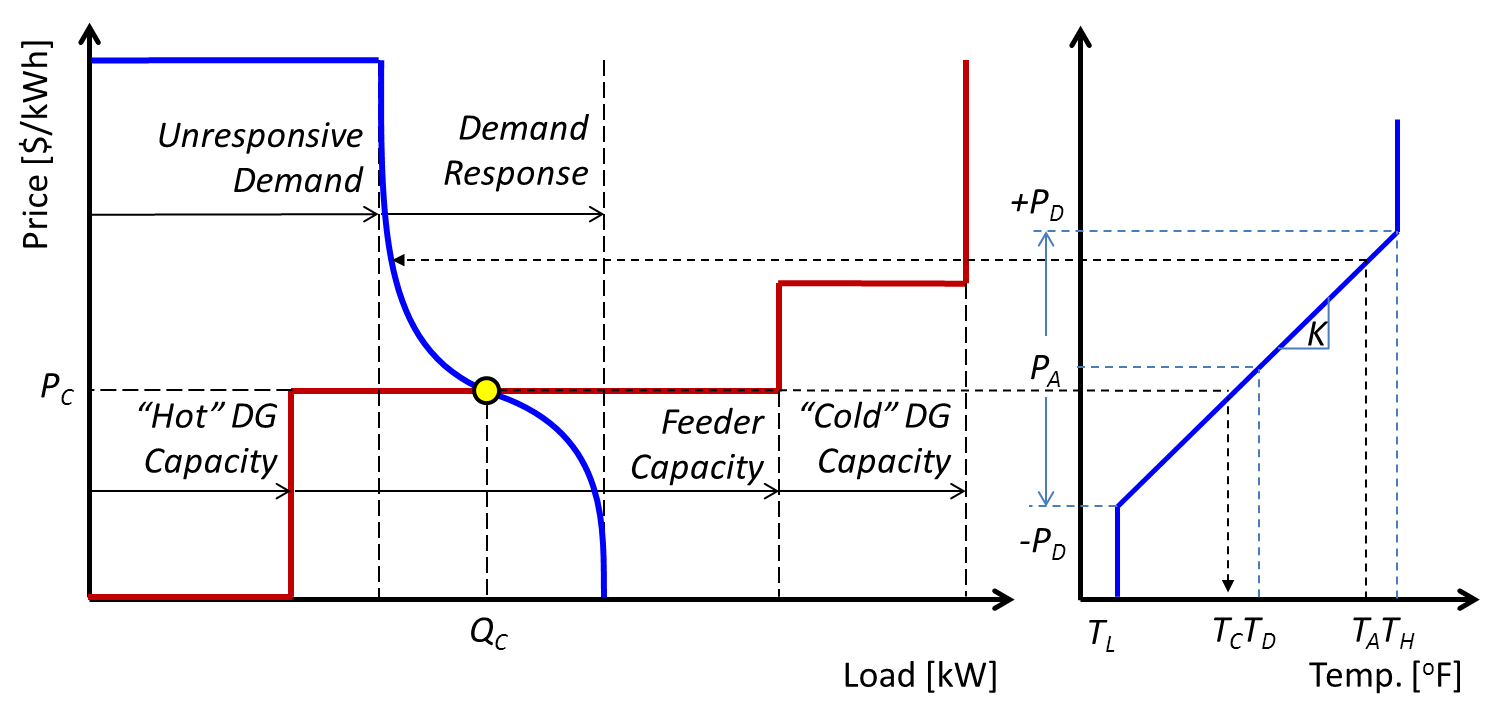
\includegraphics[width=6in]{market_clearing.png}
	\caption{Capacity market clearing (left) and thermostat bid/set for cooling conditions (right) mechanisms}
	\label{fig:market_clearing}
\end{figure}
Unresponsive load corresponds to all the other load on the feeder, including unresponsive equipment under RTP tariff, all other customers on non-RTP tariffs, services and losses.  Bids were computed by the thermostats based on measurements of the indoor air temperature such that
\begin{equation}
	P_B = \frac{k P_D }{T_M-T_D}(T_A - T_D) + P_A
\end{equation}
where $P_A$ is the long-term average price over the past 24 hours, $P_B$ is the bid price, $P_D$ is the long term price standard deviation, $k$ is the customer's comfort control setting, $T_A$ is the measured indoor air temperature,  $T_D$ is the customer's desired indoor air temperature, and $T_M$ is the maximum cooling $T_H$ or minimum heating $T_L$ indoor air temperature allowed. The quantity $K=\frac{k P_D }{T_M-T_D}$ is referred to as the demand response control gain or comfort gain in \$/$\degF$.

The supply curve was constructed from bids received by the various resources available, although in the case of the Columbus demonstration there was only the feeder supply. In the Olympic demonstration, supply included distributed generation with ``hot'' capacity representing must-run units that are already running and presumably can't or won't stop and any units that have zero marginal production cost, such as photovoltaic units.  So called ``cold'' units are those that have start-up costs included in the marginal cost and therefore are held off until the demand is sufficiently high to justify starting them.

In all existing embodiments of the transactive control system the clearing price and quantity are found at the intersection of the supply and demand curves. The clearing price is then used to change the thermostat set point such that
\begin{equation}
	T_C = T_D + K^{-1} (P_C - P_A)
\end{equation}
where $P_C$ is the cleared price, and $T_C$ is the load control set point used until the next market clearing.

The total surplus is the left-side area between the supply and demand curves. The consumer surplus accrues to consumers not willing to forgo consumption at the cleared price. The producer surplus only accrues to those producers whose costs are below the cleared price.  When the price clears above the feeder supply price, the utility collects a producer surplus from the feeder congestion. In the Columbus demonstration a congestion rebate returned the entire feeder surplus directly to the consumers while the incentive rebate compensated consumers who were curtailed as a result of congestion by diverting some of the utility's feeder surplus to pay the consumer's share of the deadweight loss caused by the withheld capacity\footnote{Some criticize this congestion rebate as self-defeating in the long run. But it was deemed necessary as a compromise that would satisfy regulators and utility managers who were concerned about whether the tariff would be revenue neutral and unfair to the participating customers. In principle producer surplus from congestion on feeders is used to finance capacity expansion. However congestion charges only occur for those customers who reside in congested neighborhoods during congested periods.  Utilities also laterally switch homes from one feeder to another to manage feeder loading so it may not be possible for a customer to ``choose'' where to live to avoid such charges.  This introduces a potential issue of fairness in the sense that customers who sign up for the tariff may perceive they are paying a greater share of capacity expansion costs through scarcity rents than other customers. The congestion rebate was introduced to avoid charging only customers on chronically congested feeders for the cost of expanding capacity, which is an asset growth cost that is normally redistributed using blended tariffs.  Customers who provide highly responsive resources are additionally compensated for curtailing under congestion through the incentive payment.}.

Although this compensation strategy does not seem likely to provide the desired long-term incentives to customers, it was hoped to have the desired effect in that it makes the bills ``feel'' more like a fixed price tariff in the long term while preserving the desired short-term incentives through savings opportunities not available to other customers. While this is consistent with the spirit of FERC Order 745, it is also quite evident that this is effectively a form of double compensation as critics of the order point out. In addition it would seem also to not be incentive compatible because a rational consumer would indicate a willingness to forgo that is higher than the true demand and one would observe a corresponding decrease in demand by the anticipated congestion fee.  The incentives would seem to be wrong both in the short and the long term.

Long-term consumer preferences played an important role in determining the short-term outcomes of the demand response system.  Newly-installed household equipment was configured with neutral defaults and customers were instructed how to enter their preferences. These preferences were an expression of the consumer's willingness to forgo comfort in the very short-term for the benefit of a decrease in cost. Preferences could be set to a variety of values by participants depending on time of day and day of week. The preference setting resulted in a discrete choice to consume or not consume at a given price and thus formed the basis of both the bid price selection based on the prevailing conditions, i.e., higher bid prices for more comfortable conditions and lower bid prices for less comfortable conditions in the home. The aggregate effect of these comfort settings give rise to a logit-shaped demand curve that changes every 5 minutes as the states of the heating and cooling systems change in response to fluctuations in the price and other endogenous behavior in the home \cite{widergren2014}.

Detailed simulations of load control using thermostats revealed some potentially significant technical problems with the first embodiment of the transactive control system used in these demonstrations. Among these was demand response dispatch control drift. When the markets cleared the measured load was initially very close to the cleared load.  However, during the five minutes that followed, before the next market clearing, the total load drifted away from the cleared load. This suggests that the 5-minute market implemented did not work well as a load dispatch ``control'' system.  The prevailing hypothesis is that the drift is the result of changes in the diversity of thermostat states induced by a common exogenous signal. These changes in the state diversity of the loads were caused by the aggregate load's initial response to the change in price \cite{pnnl2014}.  Because diversity always increases in the absence of an external forcing signal, the aggregate load tends toward the equilibrium load given the initial price signal and the prevailing conditions at the time the load is being observed. Under peak load conditions, this drift can be very significant, as illustrated in \reffig{load_control_drift}, and can only be mitigated by a) minimizing the degree to which diversity is changed by the control signal, or b) preventing the devices from changing state during the 5 minute interval between price clearings. 
\begin{figure}[ht]
\centering
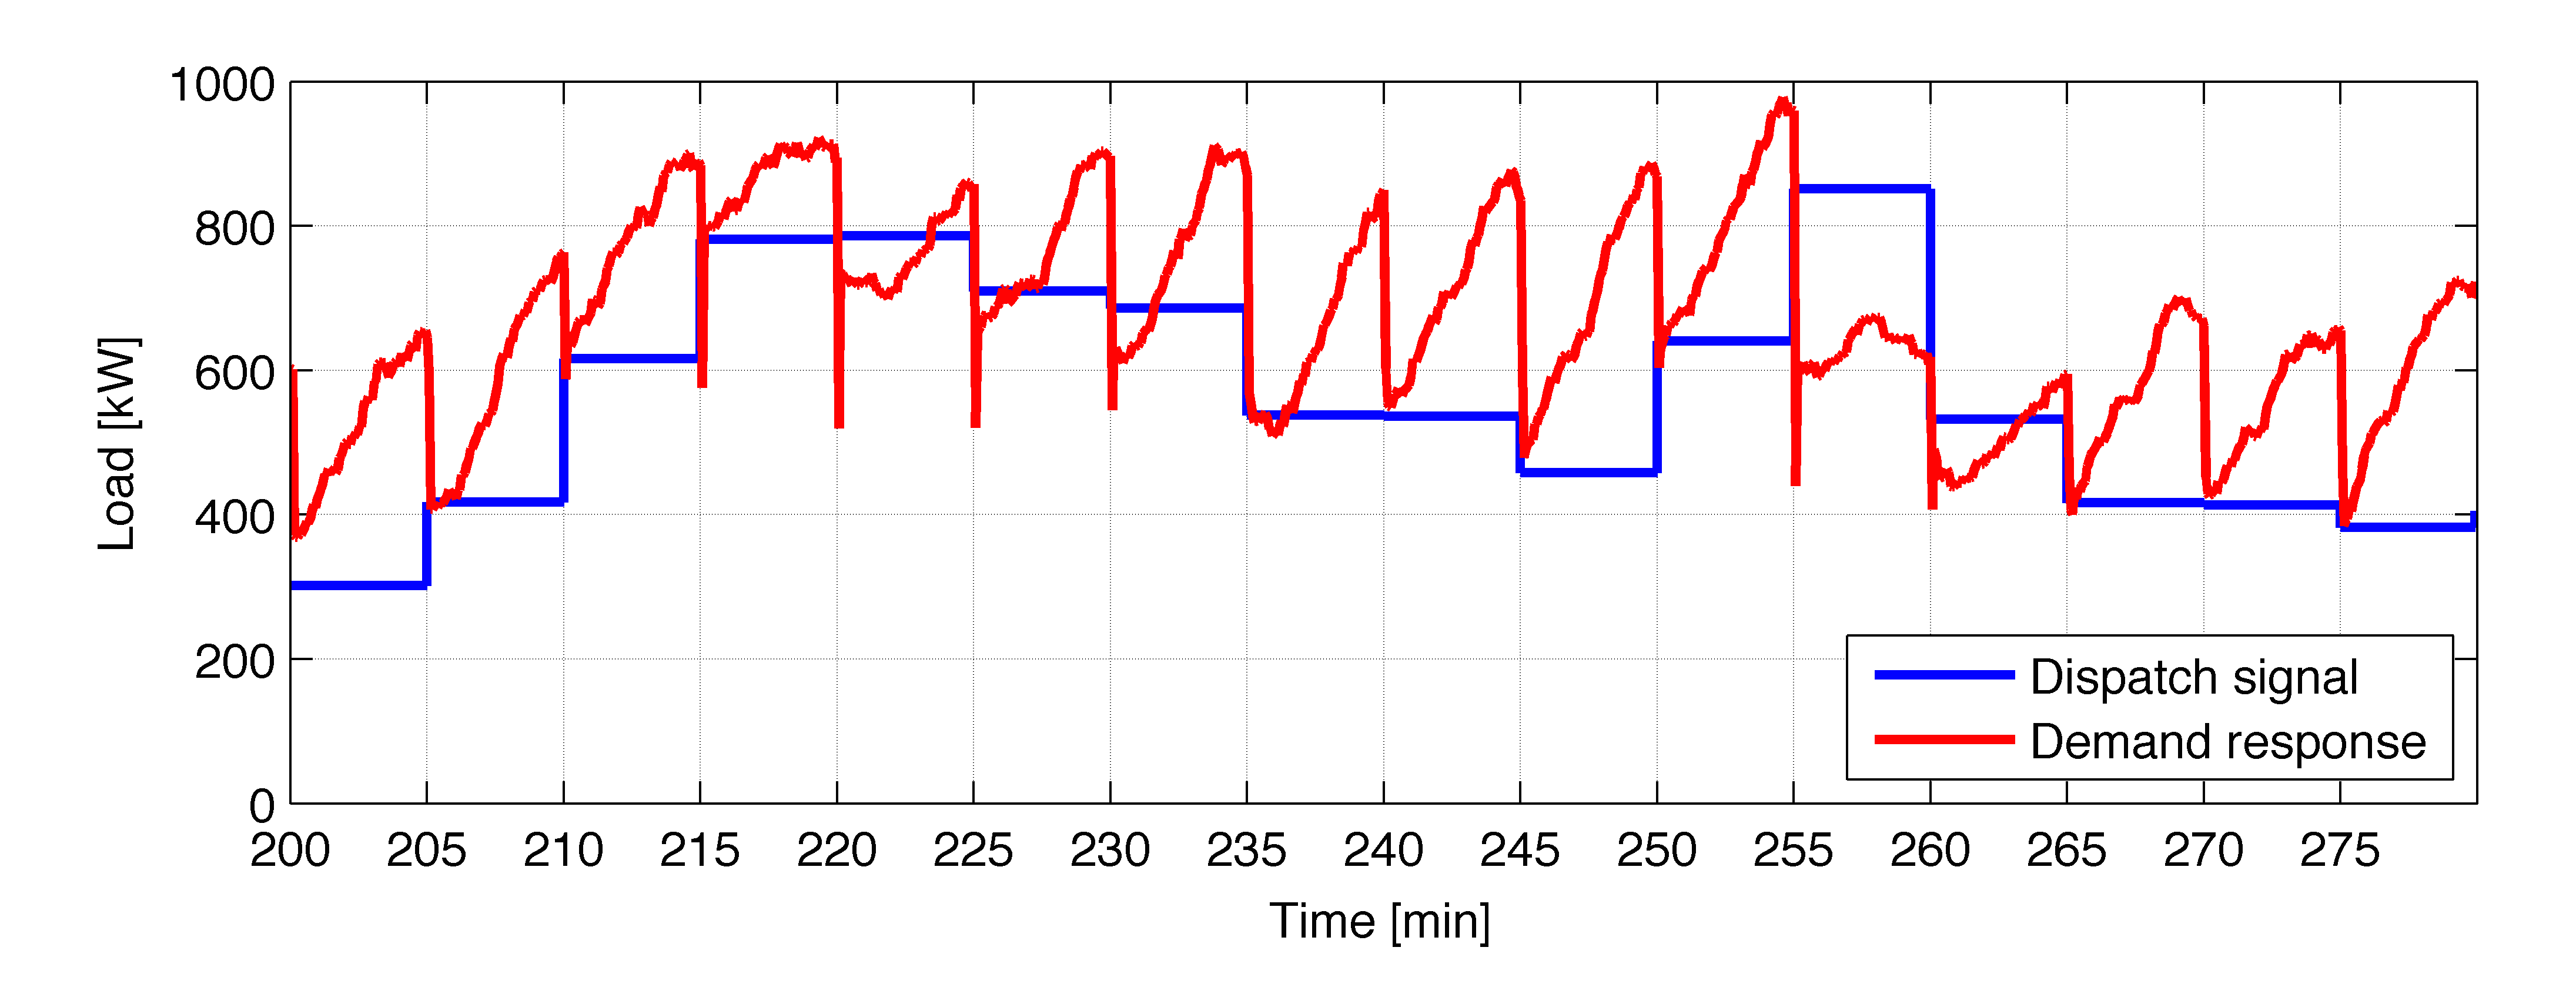
\includegraphics[width=6in]{load_control_drift.png}
\caption{Example of drift in demand response using transactive control (Data courtesy Jason Fuller, Pacific Northwest National Laboratory)}
\label{fig:load_control_drift}
\end{figure}
Because option (a) would defeat the purpose of the load control system, it would seem if diversity changes are the cause of the problem then option (b) is the only mitigation strategy available and was shown to be effective \cite{chassin2014b}.

The next phase in the development of transactive control is scaling over both physical and temporal scales. \hilight{Describe Pacific Northwest SmartGrid Demonstration project's results.}

\section{Research Objectives}
\hilight{Describe the research goals of the dissertation.}

\section{Simulation Requirements}

Simulation of transactive system requires modeling the behavior of devices interacting at time scale between 1 second and 1 hour.  Dynamic simulation engines such as PSLF, PSS/E and PowerWorld are designed to solve the electromechanical dynamics below the one second level over a period of several minutes.  In contrast production cost simulations like Plexos and PROMOD are designed to solve resource allocation at the hourly time scale are above, although they sometimes can be run at subhourly intervals given the right data. In contrast, GridLAB-D is designed to operate at the intermediate timescale where system regulation and resource dispatch intersect under control strategies like those sought for transactive systems.

\hilight{Add more of the simulation requirements.}

\section{Structure}

The overall structure of a model in the transactive module is shown in \reffig{design}.
\begin{figure}[ht]
\centering

\includegraphics[width=\textwidth]{design.png}
\caption{Transactive Module Design}
\label{fig:design}
\end{figure}

The interconnection object computes the frequency of the system based on the balance of supply and demand, the inertia and capacity of the system and the system damping coefficient.

Control areas are operated as a transactive energy market with multiple time horizons.  Control area objects compute the area control error, which is used by generators to control their power output.  Control areas are linked by tielines and have zero of more generators and loads.

Generators control one or more generating units, each of which may be a hydro, nuclear, coal, gas or wind unit.  Generators have startup and running costs that vary with time, weather and system conditions. Certain generator types response to area control error and/or implement frequency droop response. 

Loads are operated as transactive energy markets with multiple time horizons. The real-time market is similiar to the Olympic demonstrations, i.e., a distribution capacity market for customer oad and distributed generation \cite{hammerstrom2007}.
